\documentclass[conference]{IEEEtran}
\IEEEoverridecommandlockouts
\usepackage{cite}
\usepackage{amsmath,amssymb}
\usepackage{graphicx}
\usepackage{booktabs,tabularx,array}
\usepackage{tikz}
\usetikzlibrary{arrows.meta,positioning,calc,fit}
\usepackage{url}
\usepackage{balance}
\usepackage[hidelinks]{hyperref}

\newcolumntype{L}[1]{>{\raggedright\arraybackslash}p{#1}}
\newcolumntype{Y}{>{\raggedright\arraybackslash}X}

% Attack-tree styles shared by Figs. 2-4.
\tikzset{
  atroot/.style={draw, thick, rounded corners=1.5pt, align=center, font=\scriptsize\bfseries,
                 text width=8.0cm, inner sep=2.5pt, fill=black!10},
  atgoal/.style={draw, rounded corners=1.5pt, align=center, font=\scriptsize\bfseries,
                 text width=2.45cm, inner sep=2pt, fill=black!4, minimum height=0.8cm},
  atleaf/.style={draw, align=left, font=\scriptsize, text width=2.45cm, inner sep=2pt,
                 minimum height=1.25cm},
  atedge/.style={-, thin},
  ator/.style={-, thin, densely dashed},
}
% #1 root, #2-#4 sub-goals, then leaves are placed by the caller.
\newcommand{\attacktree}[9]{%
\begin{tikzpicture}[node distance=3.2mm]
  \node[atroot] (r) at (0,0) {#1};
  \node[atgoal] (g1) at (-2.92,-1.15) {#2};
  \node[atgoal] (g2) at (0,-1.15) {#3};
  \node[atgoal] (g3) at (2.92,-1.15) {#4};
  \foreach \g in {g1,g2,g3} \draw[atedge] (r.south) -- (\g.north);
  \node[font=\tiny, fill=white, inner sep=1pt] at (0,-0.47) {AND};
  \node[atleaf, below=of g1] (a1) {#5};
  \node[atleaf, below=of g2] (b1) {#6};
  \node[atleaf, below=of g3] (c1) {#7};
  \draw[atedge] (g1) -- (a1); \draw[atedge] (g2) -- (b1); \draw[atedge] (g3) -- (c1);
  #8
  #9
\end{tikzpicture}}
\newcommand{\orleaf}[3]{\node[atleaf, below=of #1] (#2) {#3};
  \draw[ator] (#1) -- node[font=\tiny, fill=white, inner sep=0.6pt]{OR} (#2);}

\hyphenation{Web-RTC edu-roam}
\makeatletter\newcommand{\tabinput}[1]{\@@input #1 }\makeatother

\begin{document}

\title{Threat-Modelling WebRTC-Based IP and Metadata Leakage on University BYOD Networks: A Campus-Specific Countermeasure Framework with an Emulated Evaluation}

\author{
\IEEEauthorblockN{Shubhi Singh and Jilagam Yatin}
\IEEEauthorblockA{\textit{School of Computer Science and Engineering}\\
\textit{Vellore Institute of Technology}\\
Vellore, India}
}

\maketitle

\begin{abstract}
WebRTC lets browsers exchange media and data directly, and to do so it gathers and shares the network addresses of the device. A university bring-your-own-device (BYOD) wireless network concentrates thousands of unmanaged personal devices on shared segments under the eduroam roaming architecture, and the operator's usual control, Wi-Fi client isolation, has published bypasses. This paper presents a threat model for that setting and tests its main recommendations in emulation. The model defines a reference campus architecture, five leakage classes, and four adversaries, builds attack trees for a lecture hall, a hostel, and a library, and maps twenty attack steps to eleven countermeasures ranked by deployment burden, enforceability, and coverage. The evaluation runs 560 browser-to-browser sessions with Chromium, Firefox, and WebKit on an emulated client segment under ten network configurations. With link-layer isolation alone, browsers that advertised raw addresses still reached each other through the gateway in 16 of 16 sessions; a gateway filter removed that path in every session. Filtering multicast DNS moved default browsers from a direct path to a relay, but only while the segment was IPv4-only behind NAT. With global IPv6 on the segment, every browser disclosed its IPv6 address in 168 of 168 sessions and connected directly over IPv6 in 56 of 56 sessions despite the multicast filter. With isolation and the gateway filter on and no relay, no session connected. A check on one laptop's physical Wi-Fi interface (60 sessions with Microsoft Edge) reproduced the emulation's NAT result: the default configuration never placed the private address in the offer, and the raw-host configuration always did. The emulation uses a Linux bridge, not Wi-Fi hardware, and desktop browser builds; mobile behaviour is taken from published measurements; the ranking remains a qualitative judgement.
\end{abstract}

\begin{IEEEkeywords}
attack trees, BYOD, client isolation, eduroam, ICE, IP address leakage, threat modelling, WebRTC, wireless network security
\end{IEEEkeywords}

\section{Introduction}
Web Real-Time Communication (WebRTC) is the browser facility behind web-based video calling, screen sharing, and peer-to-peer data transfer. To connect two browsers directly, its Interactive Connectivity Establishment (ICE) procedure gathers the addresses at which each device may be reachable and shares them with the peer~\cite{rfc8445}. A script running in a web page can read the same addresses. The result is that a page, or the other party in a call, may learn an address the user did not intend to reveal~\cite{rfc8828,rfc8826}.

The problem is old~\cite{alfannah2017,fakis2020} and only partly fixed. A cross-platform measurement published as a preprint in October 2025 found that desktop Chromium browsers now replace the local address with a multicast DNS (mDNS) name, but that Chrome and Firefox on Android still disclosed the local address on Wi-Fi and a carrier-grade NAT address on a mobile network~\cite{koysha2025}. A second study found that on networks without address translation, public addresses leak during calls even when a VPN or proxy is in use, and reported that the eduroam networks of two university campuses were such networks~\cite{nibert2025}.

A university wireless network differs from the home and enterprise networks that most of this literature assumes. Under eduroam, personally owned devices authenticate with IEEE~802.1X through a federated RADIUS hierarchy, and some belong to visitors from other institutions~\cite{rfc7593}. The operator does not own these devices and cannot require software on them~\cite{cox2017}. The same access points commonly serve an authenticated network and an open guest network at once~\cite{airsnitch2026}.

Two recent results raise the stakes. In March 2026, Sansec reported a payment skimmer that receives its code and sends stolen data over a WebRTC data channel, a path that content security policy and HTTP inspection do not cover~\cite{sansec2026}. And Wi-Fi client isolation, the control an operator would normally rely on to keep devices on one segment apart, has been bypassed in practice: by transmit-queue manipulation in 2023~\cite{framingframes2023,macstealer}, and in 2026 by a set of attacks that worked on every router and network tested, including two university networks~\cite{airsnitch2026}.

These results exist separately. The leakage studies stop at the browser. The isolation studies do not consider which application behaviour helps an attacker choose a target. Campus BYOD work stays at the level of policy and general risk~\cite{tchao2017}. An operator who wants to know what the leakage means on a campus segment, and which measures to apply first, has no single source.

This paper provides one. It builds the model by synthesis of published work and then tests the model's central recommendations in an emulated network. Its contributions are:
\begin{itemize}
\item a reference model of a campus wireless network, with five leakage classes and four adversaries, each tied to published evidence (Section~\ref{sec:model});
\item attack trees for three campus scenarios, a lecture hall, a hostel, and a library, decomposed into twenty attack steps (Section~\ref{sec:trees});
\item eleven countermeasures mapped to those steps and ranked by an explicit rule, with client isolation identified as insufficient alone (Section~\ref{sec:framework});
\item an emulated evaluation of 560 browser-to-browser sessions under ten network configurations, which measures what isolation, gateway filtering, multicast filtering, address translation, and IPv6 each change, with a check of the disclosure result on a physical Wi-Fi interface (Section~\ref{sec:eval}).
\end{itemize}
The evaluation is an emulation with desktop browsers plus a single-host check on real hardware, not a measurement on a campus network. Section~\ref{sec:limits} states what that means for the conclusions.

\section{Background}
\label{sec:background}
\subsection{ICE Candidates and Address Handling}
An ICE agent gathers host candidates from local interfaces, server-reflexive candidates from a STUN server, and relayed candidates from a TURN server~\cite{rfc8445,rfc8489}. A host candidate may be a private address, an address from the shared space used behind carrier-grade NAT~\cite{rfc6598}, or, on a network without translation, a public address.

RFC~8828 defines four address-handling modes~\cite{rfc8828}. Mode~1 enumerates all interfaces and requires user consent. Mode~2, the recommended default without consent, uses the default route and still exposes the private addresses associated with it as host candidates. Mode~3 withholds private addresses. Mode~4 forces traffic through the proxy used for HTTP. The same document names VPN exposure as its main concern.

Browsers additionally hide host addresses behind randomly generated mDNS names~\cite{mdnsdraft}. The specification for this is an expired Internet-Draft. It notes that mDNS may be disabled or limited in scope on large networks, in which case connections fall back to hairpinning or a relay, and that a malicious endpoint on the local network can still record which peers communicate.

\subsection{eduroam}
eduroam is a roaming service for research and education. The visited institution's access point acts as an 802.1X authenticator and forwards the authentication through a RADIUS proxy hierarchy to the user's home institution~\cite{rfc7593}. Credentials are visible only to the home institution. The visited institution sees the realm of an outer identity that is normally anonymous, and the device's MAC address. RFC~7593 notes that separating guest traffic from local users with VLANs is possible and widely used. It sets no requirement on address translation or on filtering of visitor traffic; those are local decisions.

\subsection{Wi-Fi Client Isolation}
Client isolation blocks direct communication between stations on the same wireless network and was introduced against attacks such as ARP spoofing~\cite{mirzoev2014}. It is not standardised. Schepers \emph{et al.} bypassed it by manipulating the frames an access point queues for a sleeping client~\cite{framingframes2023,macstealer}. Zhou \emph{et al.} analysed isolation at the encryption, switching, and routing layers and found every tested router and network vulnerable to at least one attack~\cite{airsnitch2026}. Their techniques include injecting packets through the gateway at the network layer, abusing the shared group key, and stealing the victim's switch port by connecting with its MAC address; these apply to WPA2 and WPA3 in enterprise mode as well as personal mode.

\section{Related Work}
\label{sec:related}
We searched Google Scholar with seven query formulations covering WebRTC leakage, WebRTC threat models in enterprise and BYOD settings, client-isolation bypass, campus BYOD security, and threat modelling of campus networks, and retained 41 sources after screening. Table~\ref{tab:related} summarises the clusters that bear on this paper.

\begin{table}[t]
\caption{Related Work and What It Leaves Open}
\label{tab:related}
\centering
\footnotesize
\begin{tabularx}{\columnwidth}{@{}L{1.55cm}YL{2.6cm}@{}}
\toprule
\textbf{Cluster} & \textbf{What it establishes} & \textbf{What it leaves open} \\
\midrule
Leakage measurement & Which browsers disclose which addresses~\cite{koysha2025,nibert2025,alfannah2017}; endpoint fixes~\cite{nibert2025,fakis2020}; handling modes~\cite{rfc8828} & Fixes act on the device; no network-topology analysis \\
\addlinespace
WebRTC as attack surface & Peer address exposure~\cite{tang2022,rfc8826}; egress channel~\cite{bocan2026}; data-channel skimmer~\cite{sansec2026} & Generic web or enterprise setting \\
\addlinespace
Isolation bypass & Isolation can be defeated, also on university networks~\cite{framingframes2023,airsnitch2026} & No link to application-layer leakage \\
\addlinespace
Campus BYOD & Risk assessment~\cite{tchao2017}; architecture~\cite{rfc7593}; no software on clients~\cite{cox2017} & Not tied to a specific protocol behaviour \\
\bottomrule
\end{tabularx}
\end{table}

\textit{Leakage measurement.} Koysha \emph{et al.} tested Chrome, Brave, Firefox, and Tor on Windows, Linux, and Android, with a first phase on a university Wi-Fi network, and outlined a threat model for what they call semi-trusted BYOD environments~\cite{koysha2025}. Their model classifies networks by trust level and stays at the browser; it does not decompose a campus network or rank operator-side controls. Nibert \emph{et al.} analysed desktop browsers and confined Firefox in a container as the fix~\cite{nibert2025}. Fakis \emph{et al.} used a browser extension and an HTTP gateway~\cite{fakis2020}. None of these can be imposed on a visitor's phone.

\textit{WebRTC as an attack surface.} RFC~8826 records that ICE reveals a party's address to the other party~\cite{rfc8826}. Tang \emph{et al.} show that peer-assisted video delivery exposes viewers' addresses to other viewers~\cite{tang2022}. Bocan models WebRTC pairing as an enterprise egress channel~\cite{bocan2026}, and the Sansec report shows such a channel in use by criminals~\cite{sansec2026}.

\textit{Isolation bypass.} The work in~\cite{framingframes2023,airsnitch2026} establishes that devices on a network configured for isolation can still reach or intercept each other. It treats the choice of victim as given.

\textit{Position of this paper.} The closest work is~\cite{koysha2025}, which measures on a campus network, and~\cite{nibert2025}, which observes the eduroam addressing issue. Neither builds scenario-level attack trees or an operator-facing ranking. This paper contributes that combination, and an emulated test of the operator-side controls that neither work includes.

\section{Method}
\label{sec:method}
The work is a structured synthesis in four steps, followed by an emulated evaluation.

\textit{Step 1: evidence extraction.} From each anchor source we recorded what was observed, on which platforms, and under which conditions, and separated observations from the authors' interpretation. Only observations are used as evidence.

\textit{Step 2: reference model.} We defined a campus wireless architecture from RFC~7593 and from the university deployment described in~\cite{airsnitch2026}. Every property that comes from neither source is listed as an assumption.

\textit{Step 3: attack trees.} For each scenario we wrote an attack tree in the sense of Schneier~\cite{schneier1999}: a root goal, sub-goals that must all be met, and leaf steps that are alternatives. A leaf is included only if a cited source demonstrates the step, or if it is marked as an assumption.

\textit{Step 4: countermeasure ranking.} Each countermeasure is rated on three ordinal attributes.
\begin{itemize}
\item \textit{Burden} is the larger of deployment effort and collateral impact. It is \textit{low} for a configuration change on existing equipment, \textit{medium} for a feature the equipment may not support or one that needs new operational process, and \textit{high} for a redesign or a measure that breaks legitimate use.
\item \textit{Enforcement} is \textit{network} if the operator can apply the measure to every device, \textit{managed} if it reaches only university-owned devices, and \textit{voluntary} if it depends on each user.
\item \textit{Coverage} is the number of attack steps in Table~\ref{tab:steps} that the measure blocks or exposes.
\end{itemize}
Countermeasures are sorted by burden, lowest first; then network-enforced before the others; then by coverage, highest first. The ratings are the authors' judgement from the cited sources. The rule deliberately places burden first, because the intended reader is an IT department with limited budget and no control over endpoints.

\textit{Step 5: emulated evaluation.} The recommendations that can be tested without a campus network were tested with real browsers on an emulated client segment. Section~\ref{sec:eval} gives the setup and results.

\section{Campus Threat Model}
\label{sec:model}
\subsection{Reference Architecture}
Fig.~\ref{fig:arch} shows the reference network. Each access point broadcasts three networks, as in the university deployment tested in~\cite{airsnitch2026}: eduroam with WPA2-Enterprise, a staff network with WPA2-Enterprise, and an open guest network behind a captive portal. Access points connect through a distribution switch to a gateway. A local RADIUS server authenticates local users and proxies visitors' requests to the federation~\cite{rfc7593}.

\begin{figure}[t]
\centering
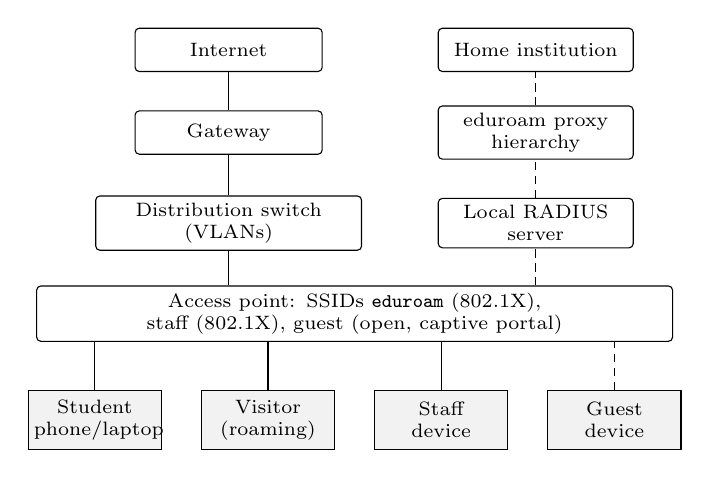
\begin{tikzpicture}[font=\scriptsize, node distance=3mm,
  box/.style={draw, rounded corners=1.5pt, align=center, inner sep=2.5pt, minimum height=0.55cm},
  dev/.style={draw, align=center, inner sep=2pt, text width=1.55cm, minimum height=0.75cm, fill=black!5}]
  \node[dev] (d1) at (-3.3,0) {Student\\phone/laptop};
  \node[dev] (d2) at (-1.1,0) {Visitor\\(roaming)};
  \node[dev] (d3) at (1.1,0) {Staff\\device};
  \node[dev] (d4) at (3.3,0) {Guest\\device};
  \node[box, text width=7.9cm] (ap) at (0,1.35) {Access point: SSIDs \texttt{eduroam} (802.1X), staff (802.1X), guest (open, captive portal)};
  \draw (d1.north) -- (d1.north |- ap.south);
  \draw (d2.north) -- (d2.north |- ap.south);
  \draw (d3.north) -- (d3.north |- ap.south);
  \draw[densely dashed] (d4.north) -- (d4.north |- ap.south);
  \node[box, text width=3.2cm] (sw) at (-1.6,2.5) {Distribution switch\\(VLANs)};
  \node[box, text width=2.2cm] (gw) at (-1.6,3.65) {Gateway};
  \node[box, text width=2.2cm] (inet) at (-1.6,4.7) {Internet};
  \node[box, text width=2.3cm] (rad) at (2.3,2.5) {Local RADIUS\\server};
  \node[box, text width=2.3cm] (fed) at (2.3,3.65) {eduroam proxy\\hierarchy};
  \node[box, text width=2.3cm] (idp) at (2.3,4.7) {Home institution};
  \draw (ap.north -| sw) -- (sw.south);
  \draw (sw) -- (gw); \draw (gw) -- (inet);
  \draw[densely dashed] (ap.north -| rad) -- (rad.south);
  \draw[densely dashed] (rad) -- (fed); \draw[densely dashed] (fed) -- (idp);
\end{tikzpicture}
\caption{Reference campus wireless architecture. Solid lines carry user traffic; dashed lines carry authentication, except the guest device, which is not authenticated by 802.1X.}
\label{fig:arch}
\end{figure}

The operator controls the access points, switches, gateway, and local RADIUS server. It controls no student, visitor, or guest device.

\textit{Assumptions.} The following are not taken from a source and may not hold at a given institution: (A1)~clients on one SSID in one building share a VLAN; (A2)~client isolation is enabled within each SSID; (A3)~address leases in residential buildings last for days; (A4)~some personal devices expose services such as file sharing on the local segment.

\subsection{Assets}
The assets are a device's local or public address, the link between an address and a person, the device's reachability from other devices, the confidentiality of its traffic, and the data a user enters in a web page.

\subsection{Leakage Classes}
Table~\ref{tab:leaks} lists the five leakage classes used in the rest of the paper, with the evidence for each. The classes describe what an attacker learns or gains; they do not depend on the campus setting.

\begin{table}[t]
\caption{Leakage Classes and Their Evidence}
\label{tab:leaks}
\centering
\footnotesize
\begin{tabularx}{\columnwidth}{@{}L{0.45cm}L{2.5cm}Y@{}}
\toprule
 & \textbf{Class} & \textbf{Published evidence} \\
\midrule
L1 & Local address to a web page & Chrome and Firefox on Android~14 disclosed the Wi-Fi address; both disclosed a carrier-grade NAT address on 4G~\cite{koysha2025} \\
L2 & Session-stable identifier & Desktop Chromium and Brave emit an mDNS name that is stable within a session~\cite{koysha2025} \\
L3 & Public address despite VPN or proxy & Observed on desktop browsers on networks without NAT; two campus eduroam networks had none~\cite{nibert2025} \\
L4 & Address to the other peer & Inherent to direct connectivity~\cite{rfc8826}; viewers exposed to each other in peer-assisted video~\cite{tang2022} \\
L5 & Covert data channel & Skimmer code and stolen data carried over a data channel outside content security policy and HTTP inspection~\cite{sansec2026} \\
\bottomrule
\end{tabularx}
\end{table}

Two limits of the evidence matter. First, the measurements in~\cite{koysha2025} did not cover VPN use, Safari, iOS, or IPv6-only networks, and are not peer reviewed. The claim that a VPN does not hide the address rests on~\cite{nibert2025} and on~\cite{alfannah2017}, not on~\cite{koysha2025}. Second, L5 comes from a vendor report about one campaign against an online shop; it shows the channel is usable, not how common it is.

\subsection{Adversaries}
\begin{itemize}
\item \textit{Remote origin (R).} Controls a web page or an embedded script that a campus user loads. Has no presence on the campus network.
\item \textit{Authenticated insider (I).} A student, staff member, or roaming visitor with valid credentials and a device on the same network as the victim.
\item \textit{Guest (G).} A person within radio range who can join the open guest network but holds no credentials.
\item \textit{Compromised page (P).} A legitimate site whose pages carry injected code, as in~\cite{sansec2026}.
\end{itemize}
An adversary who controls the infrastructure or the home institution is out of scope, as is an attack on the 802.1X authentication itself.

\subsection{Why the Campus Setting Changes the Risk}
Three properties of the reference network change what the leakage is worth to an attacker.

\textit{Density.} A device address is of little use among a handful of devices at home. In a lecture hall, hundreds of devices share an access point, and an insider who wants to reach one particular person's device must first find it. A leaked address, obtained through a link the victim opens, does that.

\textit{Persistence.} In a hostel the same device stays on the same network for months. Identifiers that are stable for a session or a lease can be collected repeatedly and joined over time.

\textit{Mixed trust on shared hardware.} The guest and authenticated networks share access points and a distribution switch. The isolation bypass in~\cite{airsnitch2026} crosses exactly that boundary.

\section{Attack Trees for Three Campus Scenarios}
\label{sec:trees}
Table~\ref{tab:scen} gives the scenarios. In each tree the three sub-goals must all be achieved, and the leaves under a sub-goal are alternatives. Table~\ref{tab:steps} lists every leaf with its source.

\begin{table}[t]
\caption{Scenarios}
\label{tab:scen}
\centering
\footnotesize
\begin{tabularx}{\columnwidth}{@{}L{1.25cm}YL{1.1cm}L{2.35cm}@{}}
\toprule
\textbf{Scenario} & \textbf{Defining property} & \textbf{Adversary} & \textbf{Main leakage} \\
\midrule
Lecture hall & Many devices on one access point for a short period & I & L1, L2, L4 \\
Hostel & Same devices on the same segment for months & R, I & L1, L2, L3 \\
Library & Guest and authenticated users on shared access points & G & L1 (supporting) \\
\bottomrule
\end{tabularx}
\end{table}

\subsection{Lecture Hall}
The attacker is a person in the room who wants to reach a specific classmate's device (Fig.~\ref{fig:hall}). The first sub-goal is to learn which of several hundred addresses belongs to the victim. A link posted to a class group suffices: the page gathers candidates without a prompt, and on Android Chrome or Firefox the candidate is the Wi-Fi address (H1). A browser-based call or file-transfer session between the two has the same effect (H2). The second sub-goal is a path to that address. It exists if isolation is absent or enforced at one layer only (H3), or it can be created by injecting through the gateway (H4) or with the group key (H5). The third sub-goal is to use the path, against a service the device exposes (H6, assumption~A4) or by intercepting the victim's downlink traffic through port stealing (H7).

WebRTC contributes only the first sub-goal. Without it, the insider can still attack devices at random, but cannot easily aim at one person.

\begin{figure}[t]
\centering
\attacktree{Reach a specific classmate's device in a lecture hall}
{Link device to person}{Obtain a path past isolation}{Act on the device}
{\textbf{H1} Victim opens a shared link; page reads the local address}
{\textbf{H3} Isolation missing or enforced at one layer only}
{\textbf{H6} Connect to a service exposed on the device}
{\orleaf{a1}{a2}{\textbf{H2} Victim joins a peer-to-peer session with the attacker}
 \orleaf{b1}{b2}{\textbf{H4} Inject packets through the gateway}
 \orleaf{b2}{b3}{\textbf{H5} Inject using the shared group key}}
{\orleaf{c1}{c2}{\textbf{H7} Steal the switch port and intercept downlink traffic}}
\caption{Attack tree for the lecture hall.}
\label{fig:hall}
\end{figure}

\subsection{Hostel}
The attacker wants to follow or repeatedly reach one resident's device over weeks (Fig.~\ref{fig:hostel}). A durable identifier comes from a call in which the public address is disclosed although the resident uses a VPN, on a segment without address translation (D1), or from a page that the resident visits repeatedly and that records the local address or mDNS name each time (D2). The identifier must then be joined across sessions, which works if the address is stable over a long lease (D3, assumption~A3) or if the page combines it with browser metadata such as platform, time zone, and screen properties (D4). The attacker then uses the linkage, locally through an isolation bypass (D5) or remotely by geolocating or flooding a public address (D6).

Here the remote origin is the main adversary, and the hostel matters because the network is the resident's home network without the address translation a home router provides.

\begin{figure}[t]
\centering
\attacktree{Track or repeatedly reach a resident's device in a hostel}
{Obtain a durable identifier}{Link it across sessions}{Use the linkage}
{\textbf{D1} Public address disclosed in a call despite VPN (no NAT)}
{\textbf{D3} Address unchanged over a long lease}
{\textbf{D5} Target the device locally through an isolation bypass}
{\orleaf{a1}{a2}{\textbf{D2} Page harvests local address or mDNS name on each visit}}
{\orleaf{b1}{b2}{\textbf{D4} Identifier joined with browser metadata}
 \orleaf{c1}{c2}{\textbf{D6} Geolocate or flood the public address}}
\caption{Attack tree for the hostel.}
\label{fig:hostel}
\end{figure}

\subsection{Library}
The attacker holds no credentials and joins the open guest network (Fig.~\ref{fig:library}). This tree follows the university experiment in~\cite{airsnitch2026}. The attacker identifies the victim's device by observing its MAC address and access point on the air (B1); a lure page that reads the victim's address can confirm which device belongs to which person (B2). The attacker then connects to the guest network using the victim's MAC address, so that the distribution switch redirects the victim's downlink traffic (B3), which is possible when the networks are not separated behind the access point (B4). Finally the attacker returns frames to the victim through the gateway or by broadcast reflection to stay unnoticed (B5) and reads what is not encrypted end to end, together with destination addresses (B6).

WebRTC leakage is not required in this tree. It appears only as B2, where it lowers the effort of choosing a victim. We include the scenario because it is the one in which the cheapest standard control fails most clearly.

\begin{figure}[t]
\centering
\attacktree{Guest intercepts traffic of an authenticated library user}
{Identify the victim's device}{Cross the network boundary}{Sustain and exploit}
{\textbf{B1} Observe MAC address and access point on the air}
{\textbf{B3} Join guest network with victim's MAC; port is stolen}
{\textbf{B5} Return frames via gateway or broadcast reflection}
{\orleaf{a1}{a2}{\textbf{B2} Lure page confirms the device--person link}}
{\orleaf{b1}{b2}{\textbf{B4} Networks share a VLAN behind the access point}
 \orleaf{c1}{c2}{\textbf{B6} Read unencrypted traffic and destinations}}
\caption{Attack tree for the library.}
\label{fig:library}
\end{figure}

\subsection{Cross-Cutting Step: Covert Data Channel}
Step X1 is independent of topology. A compromised page (adversary~P) opens a data channel to a fixed address and moves code or data over DTLS on UDP~\cite{sansec2026}. For the campus this has two consequences: users' browsers can be made to exfiltrate what they type, and monitoring that inspects only HTTP does not see it. The reported case used a non-standard UDP port; nothing prevents another from using a common one.

\begin{table*}[t]
\caption{Attack Steps, Their Basis, and the Countermeasures That Address Them}
\label{tab:steps}
\centering
\footnotesize
\begin{tabularx}{\textwidth}{@{}L{0.5cm}YL{3.9cm}L{2.6cm}@{}}
\toprule
\textbf{Step} & \textbf{Description} & \textbf{Basis} & \textbf{Countermeasures} \\
\midrule
H1 & Page opened by the victim reads the local address without a prompt & Measured on Android Chrome and Firefox~\cite{koysha2025} & C4, C5 \\
H2 & Peer-to-peer session discloses the victim's address to the attacker & \cite{rfc8826,tang2022} & C4 \\
H3 & Direct client-to-client traffic because isolation is absent or partial & \cite{airsnitch2026} & C3, C6, C9 \\
H4 & Packets injected to the victim through the gateway at the network layer & \cite{airsnitch2026} & C1, C6, C9 \\
H5 & Packets injected to the victim in frames protected by the group key & \cite{airsnitch2026} & C8, C9 \\
H6 & Connection to a service the device exposes on the segment & Assumption A4; cf.~\cite{nibert2025} & via H3--H5 \\
H7 & Downlink traffic intercepted by port stealing on the same network & \cite{airsnitch2026} & C7, C9 \\
\addlinespace
D1 & Public address disclosed during a call although a VPN or proxy is used & Desktop browsers, non-NAT network~\cite{nibert2025} & C4, C10 \\
D2 & Local address or mDNS name harvested by a page on each visit & \cite{koysha2025} & C4, C5 \\
D3 & Address remains the same across sessions & Assumption A3 & C10 \\
D4 & Identifier combined with browser metadata to link sessions & \cite{koysha2025} & C4 \\
D5 & Device targeted from the same segment through an isolation bypass & \cite{airsnitch2026} & C1, C9 \\
D6 & Public address geolocated or flooded from outside & Stated as a consequence in~\cite{nibert2025} & C10 \\
\addlinespace
B1 & Victim's MAC address and access point observed on the air & \cite{airsnitch2026} & none \\
B2 & Lure page confirms which device belongs to the victim & \cite{koysha2025} & C4, C5 \\
B3 & Guest joins with the victim's MAC address; downlink traffic is redirected & University test in~\cite{airsnitch2026} & C2, C7, C9 \\
B4 & Guest and authenticated networks are not separated behind the access point & \cite{airsnitch2026} & C2 \\
B5 & Intercepted frames returned through the gateway or by broadcast reflection & \cite{airsnitch2026} & C1, C9 \\
B6 & Unencrypted content and destination addresses read & \cite{airsnitch2026} & via B3--B5 \\
\addlinespace
X1 & Compromised page moves code or data over a WebRTC data channel & One reported campaign~\cite{sansec2026} & C6, C11 \\
\bottomrule
\end{tabularx}
\end{table*}

\section{Countermeasure Framework}
\label{sec:framework}
Table~\ref{tab:cm} lists eleven countermeasures in ranked order under the rule of Section~\ref{sec:method}. Coverage counts the steps of Table~\ref{tab:steps} in whose last column the measure appears.

\begin{table*}[t]
\caption{Ranked Countermeasures for a Campus Operator}
\label{tab:cm}
\centering
\footnotesize
\begin{tabularx}{\textwidth}{@{}L{0.55cm}L{0.5cm}L{4.4cm}L{1.0cm}L{1.35cm}L{1.05cm}Y@{}}
\toprule
\textbf{Rank} & \textbf{ID} & \textbf{Countermeasure} & \textbf{Burden} & \textbf{Enforcement} & \textbf{Coverage} & \textbf{Residual weakness} \\
\midrule
1 & C1 & Gateway rule that refuses to forward between client addresses, with IP source validation & Low & Network & 3 & Closed the gateway path in emulation (Section~\ref{sec:eval}); same-segment sessions then need a relay, and some still failed; equipment support not surveyed \\
2 & C2 & Separate VLAN for each SSID and role; guest network never bridged with authenticated networks & Low & Network & 2 & Attacks inside one VLAN remain; effect shown on one access-point model in~\cite{airsnitch2026} \\
3 & C3 & Client isolation enabled on every network & Low & Network & 1 & \textbf{Bypassable~\cite{framingframes2023,airsnitch2026}; insufficient alone.} Left the gateway path open in emulation \\
4 & C4 & User guidance: browser choice and settings, limits of a VPN, caution with shared links & Low & Voluntary & 6 & Cannot be enforced; Android defaults are weaker than desktop~\cite{koysha2025} \\
5 & C5 & Browser address-handling policy (Mode~3 or~4 of~\cite{rfc8828}) on university-owned devices & Low & Managed & 3 & Does not reach personal devices; may degrade calls \\
\addlinespace
6 & C6 & Flow telemetry at the wireless edge~\cite{rfc3176,rfc5477} to expose client-to-client flows and non-HTTP UDP flows & Medium & Network & 3 & Detects and does not prevent; sampling may miss short exchanges; needs privacy review \\
7 & C7 & MAC-spoofing safeguards: reject the gateway's MAC from wireless clients; drop a MAC seen on two networks & Medium & Network & 2 & Described as rarely available in~\cite{airsnitch2026} \\
8 & C8 & Per-client group keys, disabling shared group-addressed forwarding & Medium & Network & 1 & Affects services that rely on group-addressed traffic; needs access-point support \\
\addlinespace
9 & C9 & Per-user isolation domain (one VLAN or equivalent per client) & High & Network & 7 & Implementation challenges noted in~\cite{airsnitch2026}; scale untested \\
10 & C10 & Addressing change on client networks: translation or short-lived addresses, for IPv4 and IPv6 alike & High & Network & 3 & Moves the leak from a public to a private address; no effect if IPv6 stays global (Section~\ref{sec:eval}); redesign of the address plan \\
11 & C11 & Egress restriction on outbound UDP to known real-time services & High & Network & 1 & Breaks legitimate applications; a channel can move to an allowed port or relay \\
\bottomrule
\end{tabularx}
\end{table*}

\subsection{Reading the Ranking}
\textit{First tier, ranks 1 to 5.} These need no new equipment. C1 and C2 are the measures that the isolation literature itself recommends: placing untrusted networks in separate VLANs removes the cross-network port stealing of step B3, and network-layer filtering at the gateway removes the injection of steps H4 and B5~\cite{airsnitch2026}. C3 stays in the tier because it costs nothing where it is already supported, but it addresses a single step and is the one control with published, working bypasses. C4 has the highest coverage in the tier and the weakest enforcement: it touches every step in which the victim's browser discloses something, and it helps only the users who follow it.

\textit{Second tier, ranks 6 to 8.} These depend on features that the installed equipment may lack. C6 does not block anything; it is the only measure in the table that gives visibility into the covert channel of step X1 and into direct client-to-client traffic that should not exist when isolation holds.

\textit{Third tier, ranks 9 to 11.} C9 has the highest coverage of all eleven measures and is ranked ninth, because the rule places burden first. An operator planning a network refresh should read it as the long-term target and the first tier as what to do meanwhile. C11 ranks last: it addresses one step, partially, and blocks ordinary conferencing traffic.

\subsection{What Is Not Enough Alone}
Three common recommendations fail as single measures under this model.

\textit{Client isolation.} It blocks step H3 and none of H4, H5, H7, B3, or B5. An operator who has enabled isolation has closed the direct path and left the indirect ones.

\textit{``Use a VPN.''} On a client network without address translation, a public address can be disclosed during a call although a VPN is active~\cite{nibert2025}. The advice is still useful against other threats; it does not close L3.

\textit{Relying on browser fixes.} The mDNS replacement removes the raw address on desktop Chromium and leaves a session-stable name (L2), and the tested Android browsers still disclosed the address~\cite{koysha2025}. The operator cannot choose the browser on a personal device.

\subsection{eduroam Compatibility}
None of C1 to C3 or C6 to C11 changes the authentication exchange, so none requires cooperation from a visitor's home institution; all act on local traffic after authentication, which RFC~7593 leaves to the visited institution~\cite{rfc7593}. C4 and C5 do not reach roaming visitors at all. The anonymity of the outer identity means the visited institution usually knows a visitor's device only by realm and MAC address, which limits how far any detection under C6 can be attributed to a person.

\section{Emulated Evaluation}
\label{sec:eval}
\subsection{Questions}
Four claims of the framework can be tested without a campus network. (Q1)~Does link-layer isolation alone stop two browsers on one segment from connecting to each other, and does the gateway rule C1 close what isolation leaves open? (Q2)~Does filtering multicast suppress direct connections between browsers that hide their addresses behind mDNS names, as Section~\ref{sec:background} suggests it might? (Q3)~What does the other peer learn under translated, public, and dual-stack addressing? (Q4)~Do sessions still work when the controls are on?

\subsection{Setup}
The testbed runs on one Linux host (kernel 6.18) with network namespaces. Two client namespaces attach to ports of a bridge that stands for the client segment. A gateway namespace routes to an outside host that runs coturn~4.5.2 as STUN and TURN server. The link between gateway and outside host carries 20~ms of added delay in each direction, so that a relayed path is slower than a local one, as it is in practice.

\textit{Addressing.} In the \textit{NAT} mode clients hold private IPv4 addresses and the gateway translates; IPv6 is disabled. In the \textit{public} mode clients hold routable IPv4 addresses and nothing is translated, the situation reported for two campus eduroam networks in~\cite{nibert2025}. In the \textit{dual} mode clients have the NAT mode's IPv4 and, in addition, global IPv6 addresses that are routed without translation.

\textit{Controls.} \textit{Isolation} is bridge port isolation on both client ports, which blocks every frame between them, multicast included. \textit{mDNS filtering} drops UDP port~5353 arriving from a client port, for IPv4 and IPv6. The gateway either answers ARP on behalf of other clients and forwards between them, as private-VLAN deployments do, or drops traffic that would leave by the client interface it arrived on, which is countermeasure~C1.

\textit{Browsers.} Chromium~153.0.8010.12, Firefox~155.0, and WebKit~26.6, the builds shipped with Playwright, run headless. Seven browser configurations are used: each of the three in its default configuration; Chromium and Firefox with microphone permission granted and an audio track added, as in a call; and Chromium and Firefox in a \textit{raw-host} configuration in which mDNS obfuscation is switched off by a browser flag or preference. The raw-host configuration stands in for browsers that advertise the interface address, as~\cite{koysha2025} reports for Android. It is not an Android browser, and the WebKit build is not Safari.

\textit{Procedure.} A session starts a fresh browser in each client, opens a data channel, and exchanges offer and answer through the test harness, so signalling does not cross the emulated network. The harness waits up to 12~s for the connection and confirms it with a message echoed over the channel. It records the candidates, the selected candidate pair, and the packets from client~1 to client~2's addresses at client~1's bridge port. A session is classed as \textit{relay} if a selected candidate is relayed, \textit{direct} if frames were addressed to the peer's MAC address, and \textit{via gateway} if they were addressed to the gateway's MAC address. Ten configurations, seven browser configurations, and eight repetitions give 560 sessions. All completed without a harness error. An earlier pilot of 140 sessions without the added delay is kept with the data; where it differs, the text says so.

\begin{table*}[t]
\caption{Emulated Sessions: Path Taken, by Network Configuration and Browser Configuration. Eight Sessions per Cell. D: Direct, G: Via Gateway, R: Relay, --: No Connection}
\label{tab:results}
\centering
\footnotesize
\setlength{\tabcolsep}{4pt}
\begin{tabularx}{\textwidth}{@{}L{0.5cm}L{1.55cm}L{1.0cm}L{0.95cm}L{1.05cm}L{0.6cm}YYYYYYY@{}}
\toprule
 & \multicolumn{5}{c}{\textbf{Network configuration}} & \multicolumn{7}{c}{\textbf{Path taken (count of sessions)}} \\
\cmidrule(lr){2-6}\cmidrule(l){7-13}
\textbf{Cfg} & \textbf{Addressing} & \textbf{Isolation} & \textbf{mDNS} & \textbf{Gateway} & \textbf{Relay} & \textbf{Chromium} & \textbf{Chromium raw-host} & \textbf{Firefox} & \textbf{Firefox raw-host} & \textbf{WebKit} & \textbf{Chromium with mic.} & \textbf{Firefox with mic.} \\
\midrule
\tabinput{tab_results_body}
\bottomrule
\end{tabularx}
\end{table*}

\begin{table*}[t]
\caption{Sessions in Which the Offer Carried Client~1's Own Interface Address, by Addressing Mode and Address Family}
\label{tab:disclosure}
\centering
\footnotesize
\begin{tabularx}{\textwidth}{@{}L{3.0cm}YYYYYYY@{}}
\toprule
\textbf{Address} & \textbf{Chromium} & \textbf{Chromium raw-host} & \textbf{Firefox} & \textbf{Firefox raw-host} & \textbf{WebKit} & \textbf{Chromium with mic.} & \textbf{Firefox with mic.} \\
\midrule
\tabinput{tab_disclosure_body}
\bottomrule
\end{tabularx}
\end{table*}

\subsection{Results}
Table~\ref{tab:results} gives the path each session took and Table~\ref{tab:disclosure} what the offer disclosed. Outcomes were the same in all eight sessions of a cell except in two cells, which are named below. For a cell with eight identical outcomes the exact 95\% lower confidence bound on the underlying rate is 63\%; for 16 it is 79\% and for 56 it is 94\%.

\textit{Isolation alone leaves a path; the gateway rule closes it (Q1).} In configuration N3, isolation removed the link-layer path, and the raw-host browsers connected to each other through the gateway in 16 of 16 sessions. No attack technique was involved; this is ordinary WebRTC behaviour on a segment where the gateway forwards between clients. In N4, with the gateway rule added, none of the 56 sessions used a client-to-client path.

\textit{Multicast filtering moves default browsers to a relay, on IPv4 behind NAT only (Q2).} On the open segment N1, default Chromium connected directly in all sessions, with or without microphone permission. With the mDNS filter as the only change (N2), all 16 of those sessions used the relay. The raw-host browsers were unaffected and connected directly in 16 of 16 sessions of N2. Firefox was not uniform in N1: its default configuration connected directly in 3 of 8 sessions and with microphone permission in 7 of 8, the rest using the relay. In three captured sessions without added delay, one of the two Firefox mDNS queries was answered only on its retry about 3~s later, after the relayed pair had connected; in the pilot without added delay default Firefox used the relay in 5 of 5. WebKit used the relay in all sessions of N1. In N2 no session of default Firefox, Firefox with microphone permission, or WebKit was direct. The filter stopped having any effect once the segment carried global IPv6: in N9 all 56 sessions connected directly over IPv6.

\textit{Microphone permission did not change what was advertised.} In all 160 sessions with microphone permission, Chromium and Firefox still advertised mDNS names and no raw host address.

\textit{The addressing plan decides what a default browser discloses (Q3).} Under NAT with IPv4 only, the five configurations that keep obfuscation on never placed the interface address in the offer (0 of 200 sessions), and the raw-host browsers always did (80 of 80), whatever controls were active. Under public IPv4 addressing every session disclosed it (112 of 112). For the browsers with obfuscation it travelled as the server-reflexive candidate, which on a segment without translation is the interface address itself. Under dual-stack addressing the private IPv4 address was protected exactly as under NAT, and the global IPv6 address was disclosed in 168 of 168 sessions, again as a server-reflexive candidate. Translating IPv4 while routing IPv6 globally therefore hid nothing that identifies the device. This agrees with the observation in~\cite{nibert2025} and extends it to obfuscating browsers and to the dual-stack case.

\textit{Sessions survive the controls only with a relay, and not always then (Q4).} With isolation and the gateway rule on and no relay (N5), none of 56 sessions connected. With a relay, all 56 connected under public addressing (N7), 48 of 56 under dual-stack (N10), and 40 of 56 under NAT (N4), always through the relay. The failures are the raw-host configurations: both browsers in N4 and Firefox in N10. They reached the \textit{failed} state after about 15~s and recurred in ten further sessions with a 60~s limit. Chromium raw-host connected through the relay in the same configuration when the added delay was removed (8 of 8 sessions: five in the pilot and three in a re-run). The failure therefore depends on timing between the candidate pairs and the translating gateway. We did not determine its mechanism, and it may be specific to the Linux translation used here.

\subsection{Check on a Physical Wi-Fi Interface}
\label{sec:realhost}
The disclosure result (Q3) depends only on the browser and on the addressing of the interface, so it can be checked on real hardware without a second device. One laptop (Windows~11, Intel Wi-Fi~7 BE201 adapter associated in 802.11n mode) ran Microsoft Edge~155 headless through Playwright on its everyday Wi-Fi connection, which gave it a private IPv4 address behind NAT and only a link-local IPv6 address. Each session started a fresh browser, gathered candidates against a public STUN server, and then connected two peer connections inside the same page. Edge ran in its default configuration and in the raw-host configuration of Section~\ref{sec:eval}, 30 sessions each. Addresses were reduced to their class before they were written to disk.

In all 30 default sessions the offer carried one host candidate with an mDNS name and one server-reflexive candidate with a public IPv4 address different from the interface address; the private address never appeared. In all 30 raw-host sessions the host candidate was the private interface address, and the same server-reflexive candidate was present. No session produced an IPv6 candidate, because the interface had no global IPv6 address. All 60 loopback connections succeeded over a host pair (median gathering time 136--140~ms, median connection time 109--110~ms). This matches the NAT rows of Table~\ref{tab:disclosure} on a physical interface with a current browser build. It does not test isolation, gateway forwarding, or a second device, and it is one laptop on one network.

\subsection{Published Mobile Evidence}
\label{sec:mobile}
We could not test phones. The published evidence we found is summarised here and is not our measurement. For Android, the 2025 study reports that Chrome disclosed a LAN or carrier-grade NAT address and that Firefox, which protects the address on desktop, disclosed internal addresses on Android~\cite{koysha2025}; this is the behaviour the raw-host configuration stands for. For iOS, a 2021 test of Safari on iOS~15 observed two host candidates obfuscated with mDNS and one server-reflexive candidate, and found that with iCloud Private Relay switched on the server-reflexive candidate still carried the device's real public address until iOS~15.1~\cite{hancke2021}. A WebKit bug report from 2021, fixed in December 2022, describes Safari discarding the server-reflexive candidate when the host address is public and obfuscated~\cite{webkit233414}, which bears on the public-addressing configurations N6 to N8. None of these sources covers IPv6 on a campus segment, and none is a systematic measurement of current iOS.

\subsection{What the Results Change}
The results support three statements in the framework, sharpen one, and qualify one. They support ranking the gateway rule C1 above isolation C3: isolation by itself left a working client-to-client path for raw-host browsers. They support the statement that network controls reduce the use of a disclosed address and not the disclosure: no control changed the 80 of 80 figure for raw-host browsers under NAT. They support treating the addressing plan (C10) as the one network-side measure that changes what is disclosed. They sharpen C10: it has to cover IPv6, because a segment that translates IPv4 and hands out global IPv6 addresses disclosed a device address in every session and gave every browser a direct path that the multicast filter did not touch. They qualify C1 and C3: together these make every same-segment session depend on a relay, a web application that offers none stops working between two users on the same campus segment, and in one addressing mode some sessions failed even with a relay.

The single-host check (Section~\ref{sec:realhost}) supports the disclosure part of these statements on real hardware for one browser. Not tested: any isolation-bypass attack from~\cite{framingframes2023,airsnitch2026}, countermeasures C2 and C4 to C9 and C11, client isolation on a Wi-Fi access point, and mobile browsers.

\section{Discussion}
\label{sec:discussion}
\textit{The role of WebRTC is narrower than the headline suggests.} In two of the three trees the damaging steps belong to the isolation-bypass literature, and WebRTC supplies target selection. In the hostel tree and in step X1 it is the main mechanism. A campus operator should therefore not treat ``WebRTC leakage'' as one problem with one fix: the address disclosure is mostly a privacy and targeting issue that the network can only make less useful, while the data-channel issue is a monitoring blind spot.

\textit{Network measures reduce the value of a leak, not the leak.} No measure in Table~\ref{tab:cm} that the operator can enforce on personal devices stops a browser from disclosing an address. C1, C2, C7, and C9 make a disclosed local address harder to use. Only C10 changes what is disclosed, and it does so by substituting a less sensitive address.

\textit{Multicast filtering is a partial control that operators may already have.} The mDNS draft warns that name resolution may fail where multicast is restricted~\cite{mdnsdraft}. In the emulation this happened: default sessions moved to the relay when mDNS was filtered. The effect does not extend to browsers that advertise raw addresses, which~\cite{koysha2025} reports for Android, and it disappeared when the segment had global IPv6. It cannot be counted as a countermeasure.

\textit{IPv6 deserves the operator's attention first.} Address translation was the one network property that kept a default browser's address from the peer, and it applies to IPv4 only. A campus that runs dual-stack with global IPv6 on client segments is, for this leakage, in the position of the publicly addressed networks of~\cite{nibert2025}, whatever its IPv4 plan. The leakage measurements in~\cite{koysha2025} did not cover IPv6.

\textit{Ethics.} The paper describes attacks that are already public and adds no technique. The emulated evaluation ran on an isolated network on one computer. The single-host check exchanged packets only with a public STUN server and within the laptop itself, as any video call does; it sent nothing to other devices and recorded no address, only address classes. No data about any person or institution was collected.

\section{Limitations}
\label{sec:limits}
\begin{enumerate}
\item \textit{No live-network measurement.} The attack steps are taken from cited sources or marked as assumptions, and none was reproduced. The evaluation covers ordinary browser behaviour under four controls, not the isolation-bypass attacks.
\item \textit{Emulation, not Wi-Fi.} The client segment is a Linux bridge. Bridge port isolation stands in for Wi-Fi client isolation and does not reproduce any vendor's implementation, its weaknesses, or radio effects. The physical-interface check covers one laptop, one browser, and one IPv4-only network behind NAT, and tests disclosure only.
\item \textit{Browsers.} Only headless desktop Linux builds of Chromium, Firefox, and WebKit were used. The raw-host configuration is a switch on those builds, not an Android or iOS browser, and the WebKit build is not Safari. Mobile behaviour in Section~\ref{sec:mobile} comes from published sources, two of them informal (a blog post and a bug report), and was not measured by us. Microphone permission was granted through a fake device. Sessions used one STUN and TURN implementation, one added delay, and eight repetitions per cell, so rates between about 60\% and 100\% cannot be told apart within a cell. The failure of raw-host sessions under translation is reported and not explained.
\item \textit{Reference model, not a real network.} The architecture combines RFC~7593 with one published description of a university deployment. Assumptions A1 to A4 may be false at a given institution, and the trees change if they are.
\item \textit{Judgement-based ratings.} Burden and enforcement are ordinal ratings assigned by the authors. No cost data, vendor survey, or expert elicitation supports them. A different ordering rule, for example coverage first, would move C9 to the top.
\item \textit{Coverage counts steps, not risk.} Steps are not weighted by likelihood or impact, so a coverage of six is not twice as good as three.
\item \textit{Evidence quality.} The main leakage measurement is an unreviewed preprint that tested neither VPNs nor Apple platforms; the covert-channel evidence is one vendor report; one related-work entry~\cite{bocan2026} is an undated preprint we could not re-check.
\item \textit{Search.} The literature search used one index and was screened by the two authors without a formal protocol. Relevant work may have been missed.
\item \textit{Scope.} Attacks on authentication, rogue access points, and wired residence networks are not modelled.
\end{enumerate}

\section{Conclusion and Future Work}
\label{sec:conclusion}
This paper joined three bodies of published work, WebRTC address leakage, Wi-Fi client-isolation bypass, and the eduroam architecture, into a threat model for a university BYOD wireless network. It defined five leakage classes and four adversaries, decomposed three campus scenarios into twenty attack steps, and ranked eleven countermeasures for an operator who cannot touch the endpoints. Under a rule that puts deployment burden first, gateway filtering and VLAN separation rank highest, per-user isolation is the strongest measure and the most expensive, and client isolation is a baseline that must not be relied on alone. An emulation with 560 browser sessions, and a 60-session check on a physical Wi-Fi interface for the disclosure result, agreed with the ranking on the points it could test and added two findings. Isolation alone left a path through the gateway for browsers that advertise raw addresses, and the gateway rule closed it. Address translation, not mDNS obfuscation or multicast filtering, decided whether a default browser's address reached the peer, and global IPv6 on the client segment undid that protection in every session.

The next steps are to repeat the evaluation on Wi-Fi access points and with Android and iOS browsers; to reproduce the leakage measurements on a campus network with the operator's approval, including VPN cases; to check assumptions A1 to A4 against real deployments; to find the mechanism of the relay failures under translation; and to replace the ordinal ratings with estimates from campus network administrators.

\balance
\bibliographystyle{IEEEtran}
\bibliography{references}

\end{document}
